\chapter{Mecánica Celeste}

\section{Introducción}
La mecánica celeste es la rama de la astronomía que se ocupa del movimiento de los objetos celestes, como planetas, satélites y cometas. 

Consideremos dos cuerpos de masas $m_1$ y $m_2$ con vectores de posción $\rn_1$ y $\rn_2$ aislados en un sistema inercial ccon origen en su centro de masas $\rn_c$. 

El sistema está compuesto por 6 EDOs no lineales, autónomas y de 2º orden (que sean autónomas significa que no dependen del tiempo explícitamente). 

Estudiamos el movimiento el movimiento relativo $\rn=\rn_1-\rn_2$. Así podemos reescribir el sistema como

\begin{equation}
    \ddot{\rn} = - \frac{\mu}{r^3}\rn
\end{equation}
donde $\mu$ es la \textbf{masa reducida} definida por $\mu=G(m_1+m_2)$. El sistema así escrito está compeusto por 3 EDOs no lineales y autónomas de segundo orden, que podeos reescribir como un sistema de 6 EDOs de orden 1:

\begin{equation}
    \dot{\rn} = \vn \tquad \dot{\vn}= - \frac{\mu}{r^3}\rn
\end{equation}
La solución del problema de Kepler es el movimiento que satisface la ecuación anterior $\rn(t)$., y también satisfará $\ddot{\rn}=-\frac{\mu}{r^3} \rn$. Encontramos tres canti dades conervadas: momento angular, energía y vector excéntrico. 

\begin{itemize}
    \item Definimos el \textbf{momento angular} $\cn = \rn \wedge \vn$.
    \item La \textbf{energía} se define como $h=\frac{v^2}{2}-\frac{\mu}{r}$. Se define como la energía por unidad de masas, ya que al pasar al problema de masa reducida aparece así.
    \item El \textbf{vector excéntrico} se define como $\en = \frac{1}{\mu} \vn \times \cn - \frac{\rn}{r}$. 
\end{itemize}
\begin{Anotacion}
    \textcolor{red}{ Hablar del vector excéntrico, por que se usa este en vez de el momento lineal en el problema de dos cuerpos, cual es el significado físico, de donde viene, hablar de la sobredeterminación de los momentos angulares }
\end{Anotacion}

En lugar de utilizar el momento lineal total \( \mathbf{P} \), el momento angular \( \mathbf{L} \) y la energía \( E \), es más conveniente emplear \( \mathbf{L} \), \( E \) y el vector excéntrico \( \mathbf{e} \) para describir las órbitas en el problema de dos cuerpos. Esta elección se debe a que estas cantidades conservadas permiten una parametrización geométrica más clara de la órbita.

\begin{itemize}
    \item El momento angular \( \mathbf{L} \) define el \textbf{plano orbital}.
    \item El vector excéntrico \( \mathbf{e} \) determina la \textbf{orientación dentro del plano}.
    \item La energía \( E \) fija el \textbf{tamaño de la órbita}. 
\end{itemize}

La ecuación de la órbita en coordenadas polares está dada por:

\begin{equation}
    r = \frac{p}{1 + e \cos\theta},
\end{equation}

donde \( p \) es el semilatus rectum de la trayectoria, dado por:

\begin{equation}
    p = \frac{L^2}{\mu G M}.
\end{equation}

Esta parametrización facilita el análisis de las órbitas en términos de sus propiedades geométricas y permite obtener soluciones explícitas del problema de Kepler de manera más intuitiva.


\begin{Anotacion}
    \textcolor{red}{Hizo todo el cálculo sobre como obtener $\en$ (demostración de que se conserva), como obtener $e$ y su relación con la energía (fácil, pero zzz).}
\end{Anotacion}

\section{Solución general y orbitas cónicas}

Llagamos a las solución general:

\begin{equation}
    r(f) = \frac{c^2 / \mu}{1+e\cos (f)}
\end{equation}
donde $f \in [0,2\pi)$ es ángulo de los vectores $\en$ y $\rn$. Siendo $l$ el semilatus rectum, que es la distancia entre el foco de la elíptica y la elíptica en la recta perpedicular a la daigonal mayor. La ecuación polar de una sección cónica es 

\begin{equation}
    r(f) = \frac{l}{1+e\cos(f)}
\end{equation}
En función de $e$ tendremos varios tipos de movimiento: 

\begin{itemize}
    \item $e=0$. Movimiento circular
    \item $0<e<1$. Movimiento elíptico.
    \item $e=1$. Movimiento parabólico.
    \item $1<e$. Movimiento hiperbólico.
\end{itemize}
Las soluciones al problema de kepler son movimietos a lo largo de cónicas. El tipo de cónica lo determina $e$, y también $h$, en virtud de la relación

\begin{equation}
    e^2 = 1 + \frac{2}{\mu^2} c^2 h
\end{equation}
Podemos ver aquí que $e$ es mayor, menor o igual que uno depende únicamente de si $h$ es positivo, negativo o cero, por lo que la energía también nos permite calcular que tipo de movimiento tiene nuestra órbita.
\begin{Anotacion}
    \textcolor{red}{Insertar dibujo sobre la semilaptus rectum. Tambíen hizo un dibujo, donde el eje x es la energía, el eje y el momento angular, y reprsento cual es el tipo de órbita en función de la región de dicho espacio de fases (elíptico, hiperbólico, parabólico, colisión...)}
\end{Anotacion}

\section{Leyes de Kepler}

Hay 3 leyes de Kepler:

\begin{itemize}
    \item Ley de las órbitas: los planetas se mueven en órbitas elípticas, con el Sol en uno de los focos de la elipse. 
    \item Ley de las áreas: la línea que conecta un planeta y el Sol barre áreas iguales en tiempos iguales.
    \item Ley de los períodos. El cuadrado del período orital de un planeta $T$ es proporcional al cubo de la distancia media del planeta al Sol: 
    \begin{equation}
        T^2 = \frac{4\pi^2}{\mu}a^3
    \end{equation}
    donde $a$ es el semieje mayor de la elipse, que es igual al promedio entre las distancias y en afelio $r_a$. 
\end{itemize}
Definimos el \textbf{perhelio} como $f=0$, el punto mas cercano del centro de la órbita, y el \textbf{afelio} como $f=\pi$, el punto más alejado del centro de la órbita. Asi, tenemos que 

\begin{equation}
    r_{\text{perhelio}} = \frac{c^2/\mu}{1+e} = a(1-e) \tquad r_{\text{afelio}} = \frac{c^2/\mu}{1-e} = a(1+e)
\end{equation}
Definimos $a=r_p+r-a/2$. Para otro tipo de órbitas se define periapsis y apoapsis como los puntos 

\section{Elementos orbitales}

Son 6 parámetros que definen la órbita de un cuerpo celeste con respecto a un plano de referencia, así como la posición del cuerpo en la órbita. Tres de ellos ya los hemos estudiado: semieje mayor $a$ (distancia media del cuerpo al foco), excentricidad $e$ (medida de la forma de la órbita) y anomalía verdadera $f$ (posición del cuerpo en su órbita en un momento dado). En algunas ocasiones, en lugar de la anomalía verdadera, se emplea el tiempo de paso por el periastro ($\tau$), la anomalía media ($M$) o la longitud media ($L$).

\begin{Anotacion}
    \textcolor{red}{ Se está centrnado bastante en las características de la anomalía media (dice que varía a velocidad constante). Hablar de las demas cosas, significado, uso, razón. (Video de true anomaly vs mean anomaly), así vemos la relación entre ellas. }
\end{Anotacion}

Además tenemos los siguientes elementos orbitales. Se define $\Nn$ como el vector nodo ascendente tal que $\Nn=\hnz \wedge \cn$. Apunta en dirección al nodo ascentende y está contenido en ambos planos. 

\begin{itemize}
    \item Inclinación $i$. ángulo entre el plano de la órbita y el plano de referencia.
    \begin{equation}
        \cos (i) = \frac{\cn \cdot \hnz}{|\cn||\hnz|}
    \end{equation}
    \item Longitud del nodo ascendente $\Omega$. Ángulo medido en plano de referencia desde la dirección referencia hasta la dirección del modo ascendente.
    \begin{equation}
        \cos (\Omega) = \frac{\Nn \cdot \hnx}{|\Nn||\hnx|}
    \end{equation}
    \item Argumento del periastro $\omega$. (Periastro y periapsis es el mismo concepto, pero la segunda para conicas generales y el primero para cuando implican astros). 
    \begin{equation}
        \cos (\omega) = \frac{\Nn\cdot \en}{|\Nn||\en|}
    \end{equation}
\end{itemize}
Resumen los elementos $i,\Omega$ de terminan el plano de la órbita con respecto al de referencia., mientras qeu $e,\omega$ y $a/c$ ($a$ si $e<1$ o $c$ si $e\geq1$) determiann la forma y orientación de la órbita en el plano de órbita  El elemento $f$ determinar la posición del campo en su órbita.


\section{Ejercicios}

\tcbstartrecording
\begin{texercise}
    
    \tcblower
    Tenemos que demostrar que el vector excentricidad lleva el sentido hacia la periapsis. 
    

    \begin{minipage}{.45\textwidth} 	
        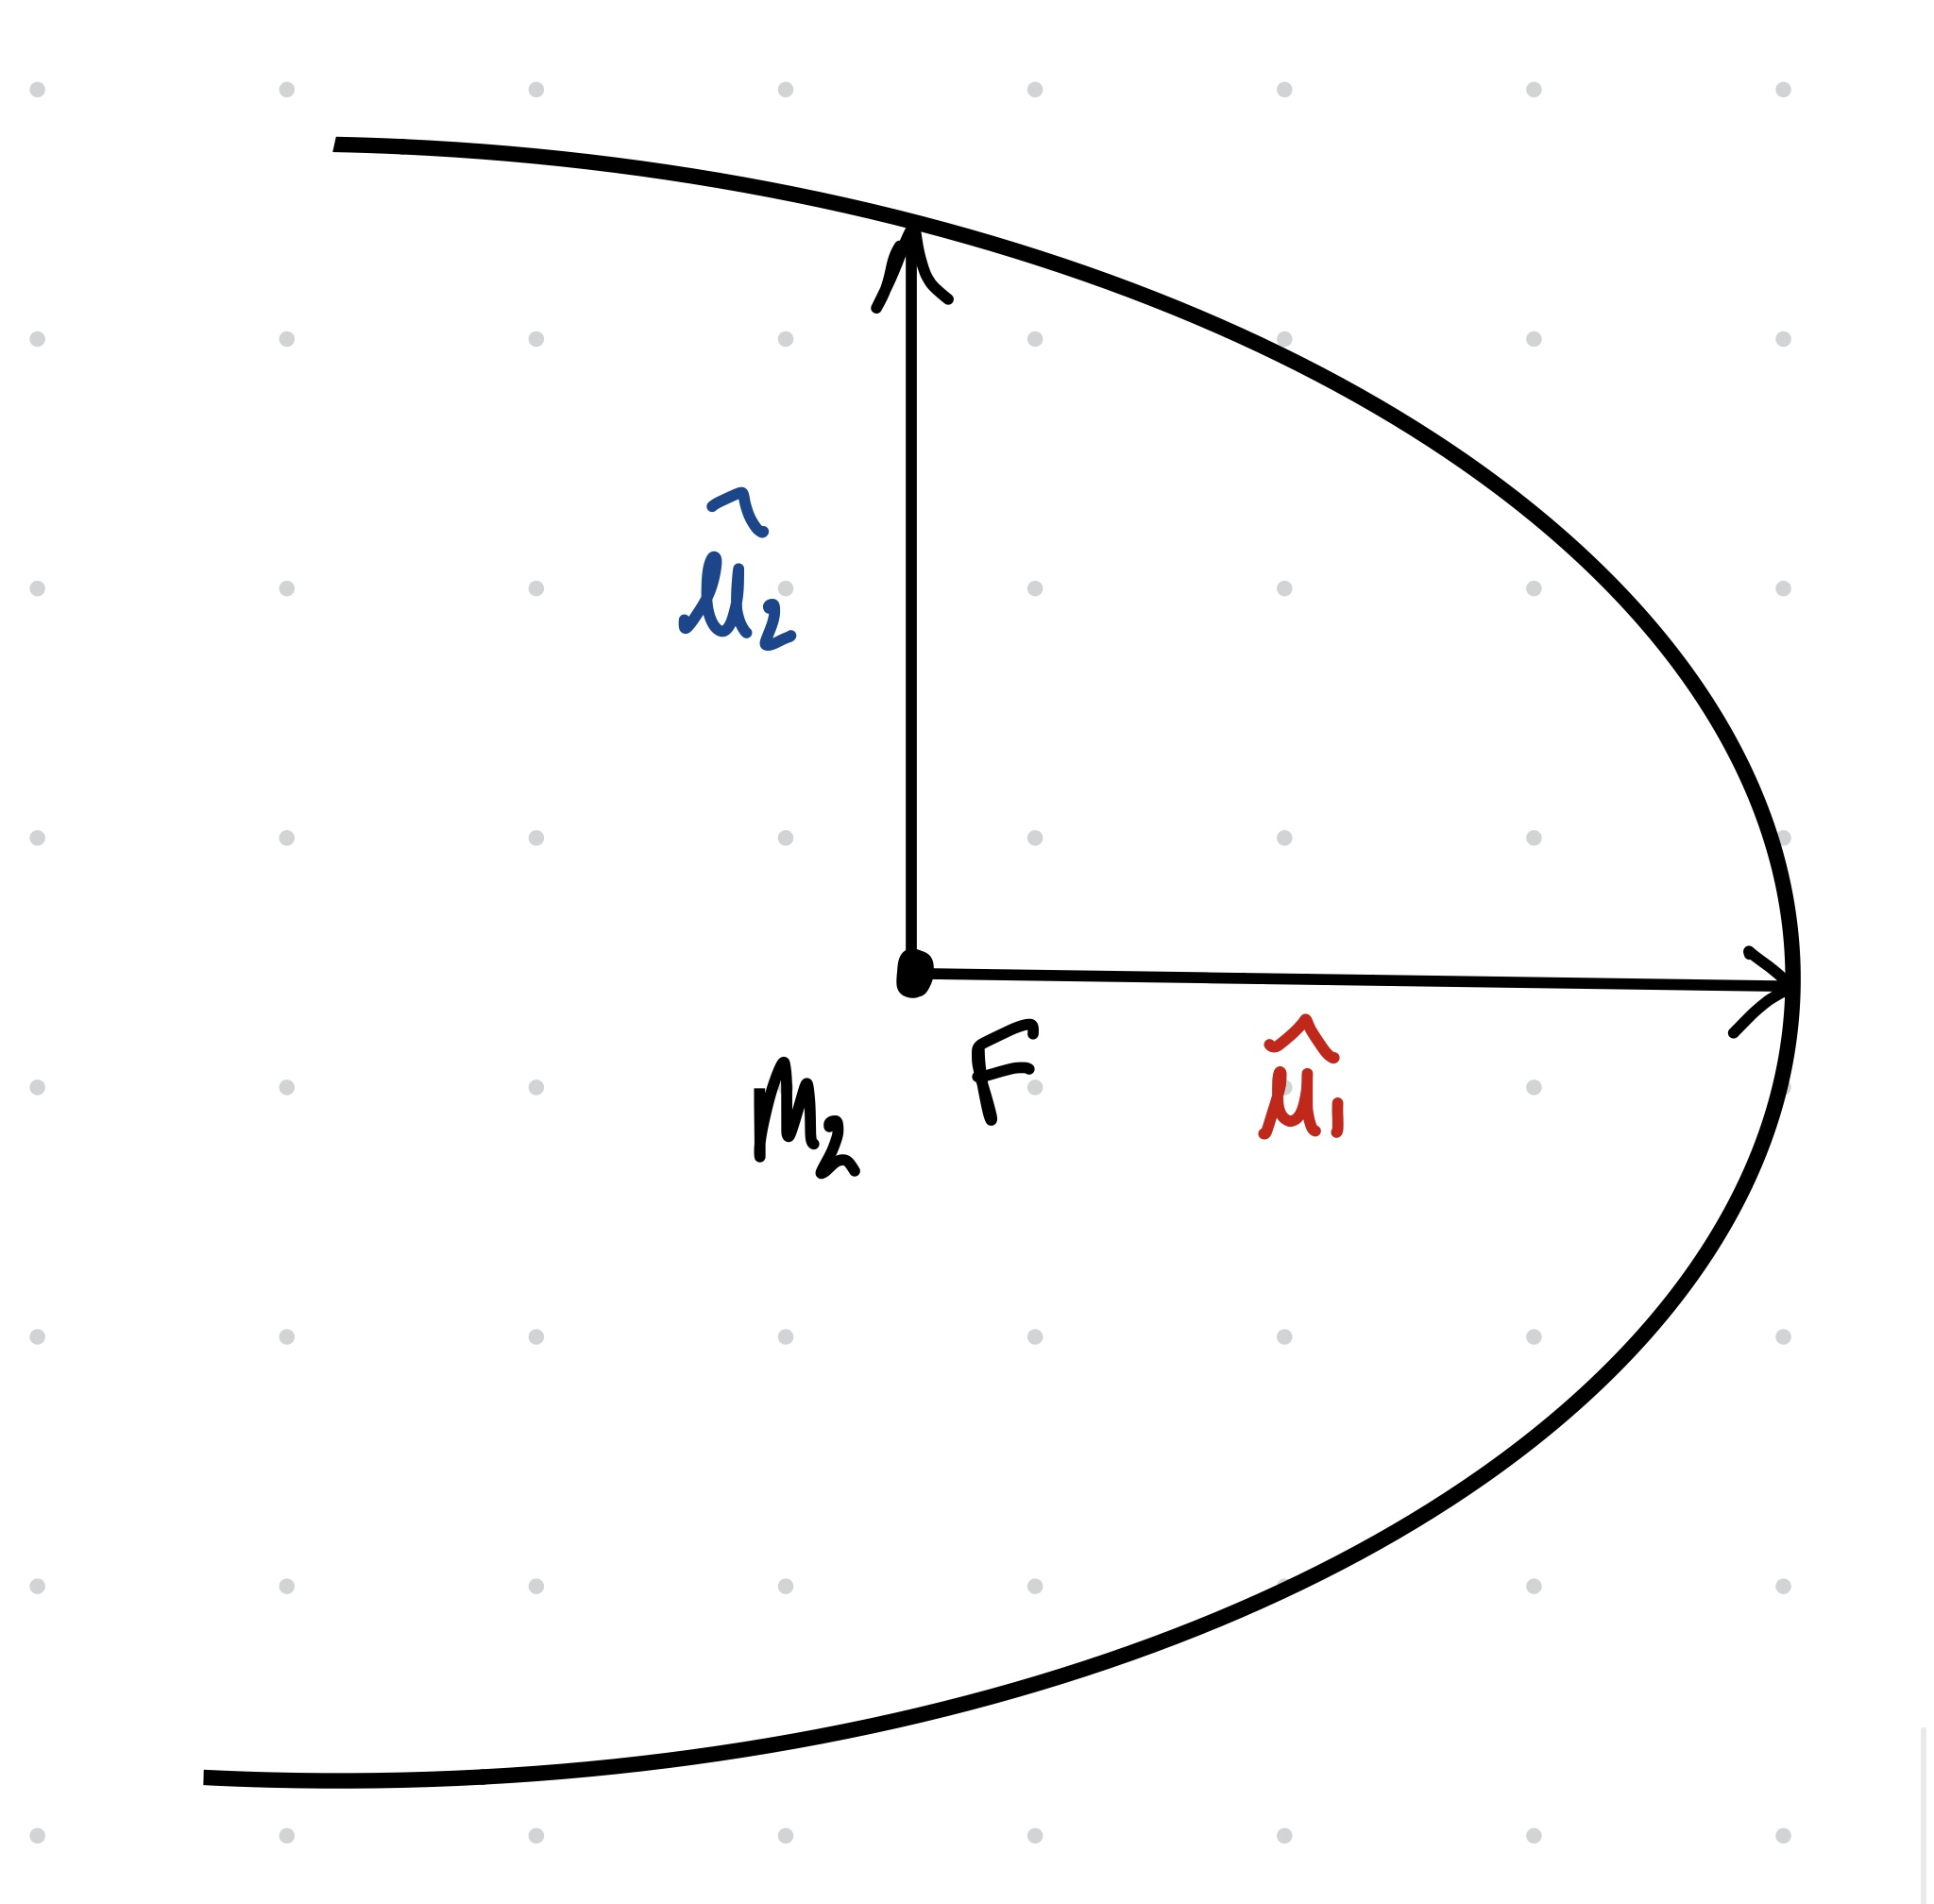
\includegraphics[width=0.8\textwidth]{Cuerpo/Imagenes/02_Ejercicio_1_1.jpg}
    \end{minipage}	\hfill
    \begin{minipage}{0.45\textwidth} 
        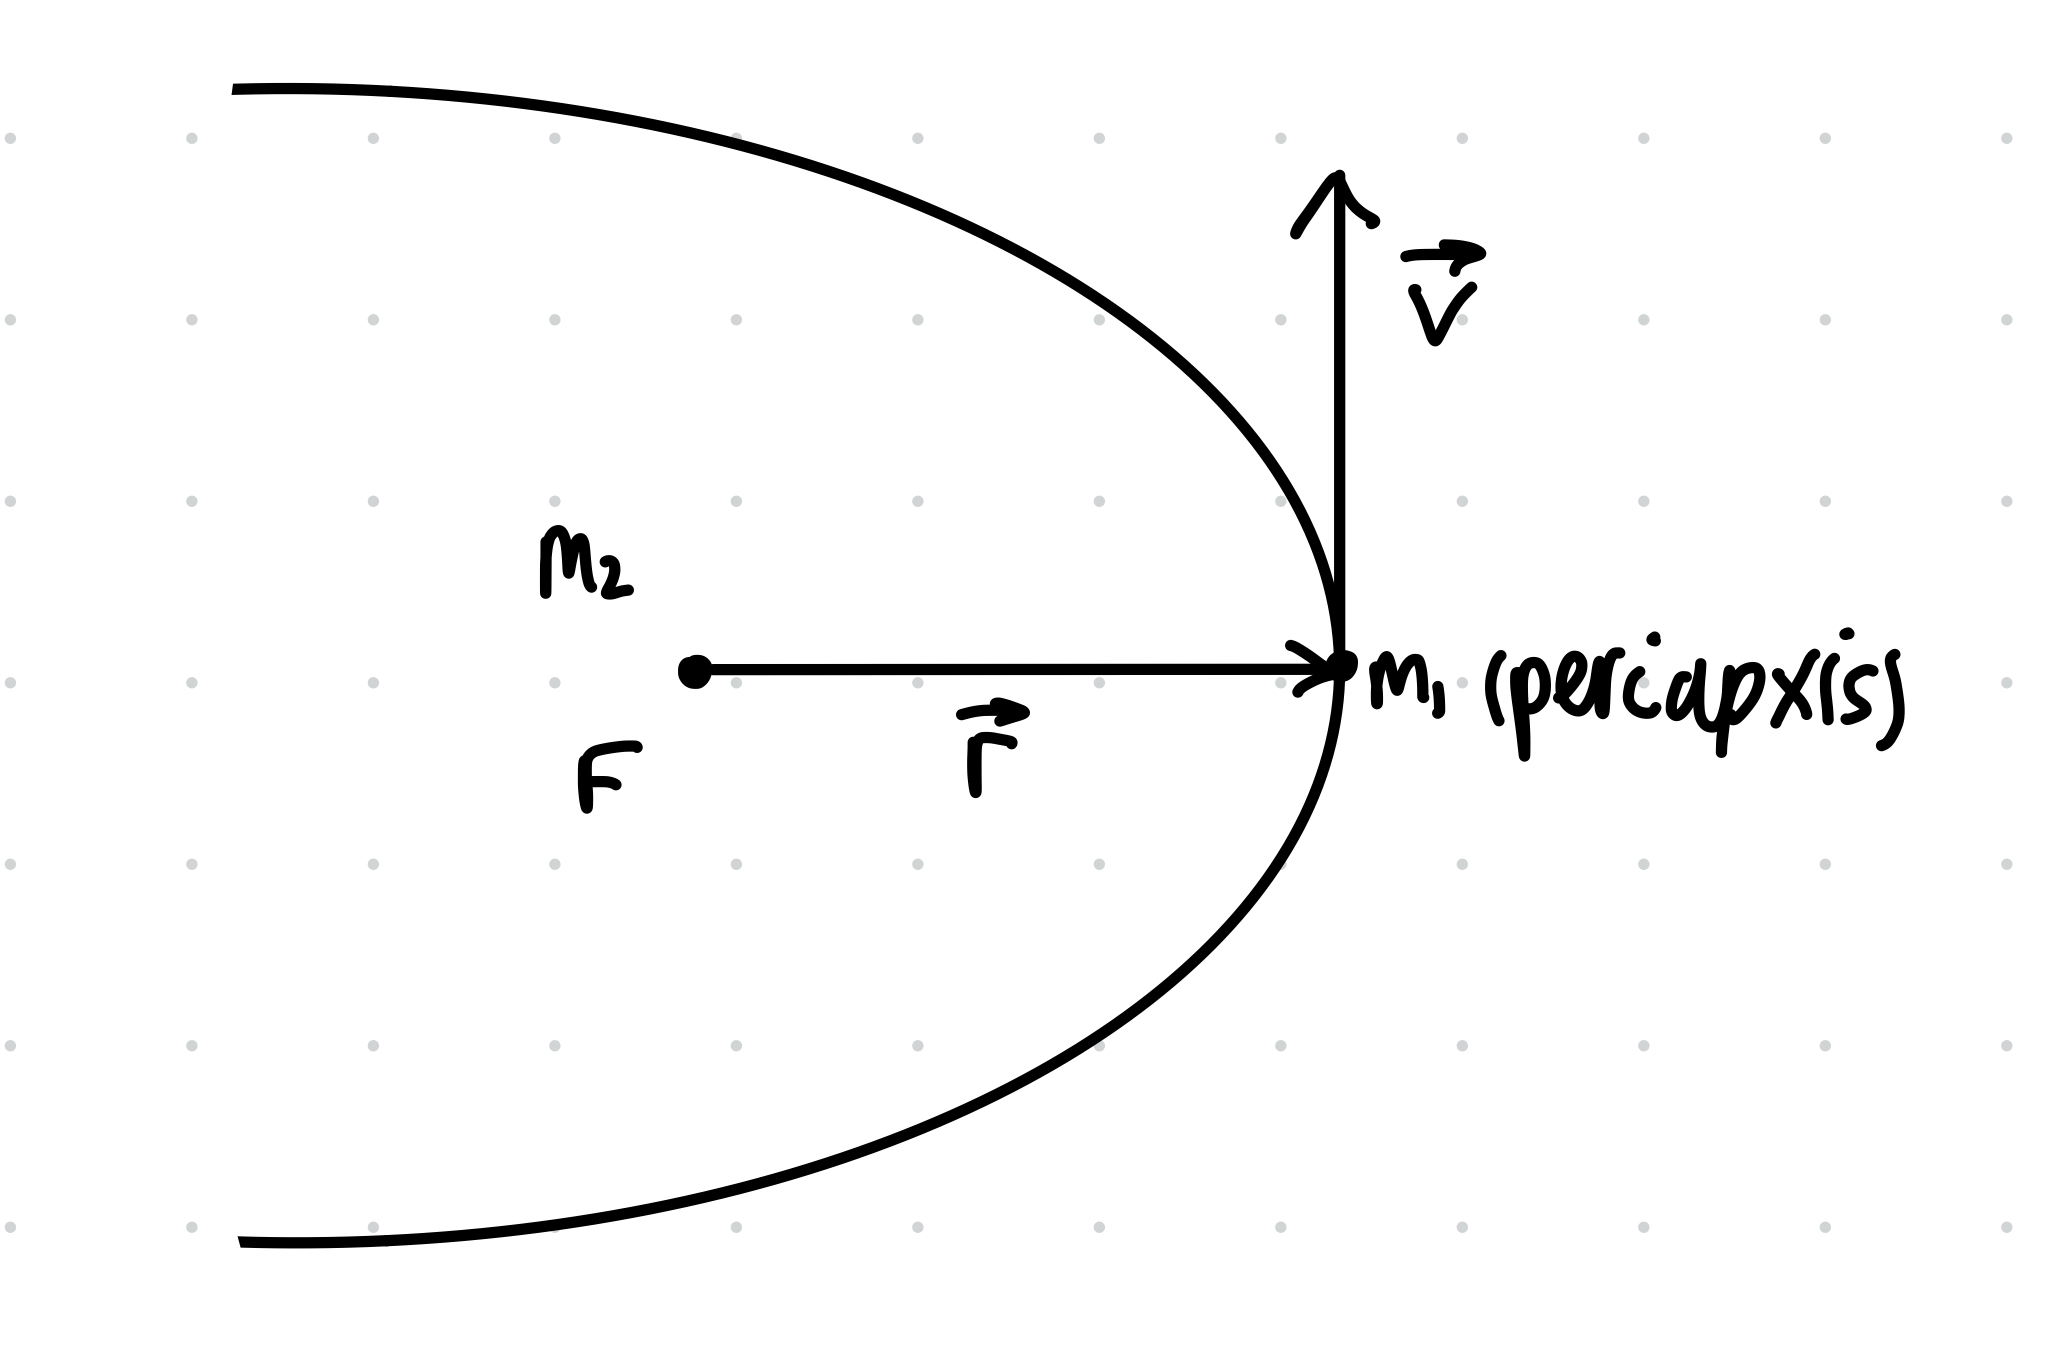
\includegraphics[width=1.0\textwidth]{Cuerpo/Imagenes/02_Ejercicio_1_2.png}
    \end{minipage}

    Tenemos que $\cn=c\hnu_3$ donde $\hnu_3=\hnu_1\wedge\hnu_2$. Supongo que $m_2\gg m_1$. Entonces:

    \begin{equation}
        \rn_c \simeq \rn_2 = 0 \tquad \rn_1 = \rn \tquad \vn = v \hnu_2
    \end{equation}
    Y por tanto $\en=\frac{1}{\mu} (\vn \wedge \cn) - \frac{\rn}{r}$. Ahora hacemos que 

    \begin{equation}
        \vn \wedge \cn = \begin{vmatrix}
            \hnu_1 & \hnu_2 & \hnu_3 \\
            0 & v & 0 \\
            0 & 0 & c
        \end{vmatrix} = v c \hnu_1
    \end{equation}
    Y por tanto:

    \begin{equation}
        \en = \frac{vc}{\mu} \hnu_1 - \hnu_1 \Rightarrow \en = \ccorchetes{\frac{vc}{\mu}-1}\hnu_1
    \end{equation}
    quedando demostrado que lleva el sentido de la periapsis. 
\end{texercise}

\begin{texercise}
    Hola
    \tcblower
    Tenemos la ecuación para conocer el ángulo:

    \begin{equation}
        r(f) = \frac{c^2/ \mu}{1+e\cos(f)}
    \end{equation}
    Cuando $e=1$ tenemos perihelio $f=0$. El valor de $r_p = c^2/2\mu$. El valor de la masa reducida $$\mu=G(m_{\text{sol}}+m_{\text{cometa}})\simeq G m_{\text{sol}} = 2.95\cdot 10^{-4} \ua^3/d$$(ddespreciamos la masa del cometa).Ahora calculamos 

    \begin{equation}
        c=|\rn\wedge\vn|=0.015 \*ua^2/
    \end{equation}
    de lo que puedo obtener el valor de $r_p$:
    \begin{equation}
        r_p = \frac{c^2}{2\mu} = 0.379 \ua
    \end{equation}
\end{texercise}
\tcbstoprecording

\section{{Soluciones}}

\tcbinputrecords
